% !TEX program = pdflatex
% !BIB program = bibtex
% !TEX encoding = UTF-8 Unicode
% !TEX spellcheck = en_us
\documentclass[10pt,sigconf]{acmart}

\usepackage{booktabs} % For formal tables

\graphicspath{{figure/}{figures/}}

% Copyright
%\setcopyright{none}
%\setcopyright{acmcopyright}
%\setcopyright{acmlicensed}
\setcopyright{rightsretained}
%\setcopyright{usgov}
%\setcopyright{usgovmixed}
%\setcopyright{cagov}
%\setcopyright{cagovmixed}


% DOI
\acmDOI{10.475/123_4}

% ISBN
\acmISBN{123-4567-24-567/08/06}

%Conference
\acmConference[CR for Nano'21]{AzuNet Seminar}{July 2021}{Lübeck, Germany} 
\acmYear{2021}
\copyrightyear{2021}

\acmPrice{15.00}


\begin{document}
\title{Computational Requirements for Nano-machines}
%\titlenote{Produces the permission block and copyright information}
%\subtitle{Extended Abstract}

\author{Melanie Badura}
\orcid{1234-5678-9012}
\affiliation{
  \institution{Universität zu Lübeck}
  \streetaddress{Ratzeburger Allee 160}
  \city{Lübeck}  
  \postcode{23560}
}
\email{melanie.badura@student.uni-luebeck.de}




% The default list of authors is too long for headers}
\renewcommand{\shortauthors}{M. Badura et al.}


\begin{abstract}
This paper is a short paper for "Computational Requirements for 
Nano-Machines: There is limited Space at the bottom"\cite{lau2017computational}.
The premise is to define the complexity of scenarios done at a nanoscale, which most research omitted.
The problems we filter out of these scenarios sort into the complexity classes $AC^0$, $NC^1$, L.
\end{abstract}

%
% The code below should generate by the tool at
% http://dl.acm.org/ccs.cfm
% Please copy and paste the code instead of the example below. 
%
\begin{CCSXML}
<ccs2012>
 <concept>
  <concept_id>10010520.10010553.10010562</concept_id>
  <concept_desc>Computer systems organization~Embedded and cyber-physical systems</concept_desc>
  <concept_significance>500</concept_significance>
 </concept>
 <concept>
  <concept_id>10010520.10010575.10010755</concept_id>
  <concept_desc>Computer systems organization~Sensor networks</concept_desc>
  <concept_significance>300</concept_significance>
 </concept>
 <concept>
  <concept_id>10003033.10003083.10003095</concept_id>
  <concept_desc>Networks~Network reliability</concept_desc>
  <concept_significance>100</concept_significance>
 </concept>
</ccs2012>  
\end{CCSXML}


\ccsdesc[500]{Computer systems organization~Embedded and cyber-physical systems}
\ccsdesc[300]{Computer systems organization~Sensor networks}
\ccsdesc[100]{Networks~Network reliability}

% We no longer use \terms command
%\terms{Theory}

\keywords{nanonetworks; computational complexity; space-complexity}


\maketitle

\section{Introduction}
For years researchers are talking about using nano-machines to create solutions in medicine and other subjects. Such a machine should be able to communicate and sense/act. Thus computational power is also a big issue.
Because Nano-machines are small, one question is how to implement these capabilities. 
While many researchers already deal with communication technology \cite{akyildiz2008nanonetworks}, they usually leave out computational capabilities.
In this paper, there is an attempt to provide a general analysis of the computational capability of nano-machines.
Since the capabilities of nano-machines vary widely, from nanoparticles with no computational capabilities to microprocessors \cite{cobo2010bacteria}, nano-machines divide into three groups according to complexity theory.
We define the three groups by analyzing the tasks that nano-machines handle.



\section{Problems and their complexity classes}
\begin{table}[h!]
  \begin{tabular}{ p{1.5cm}|p{2cm} p{2cm}}
    \hline
    %\multicolumn{5}{|c|}{MSE} \\
    Machine & \multicolumn{2}{c}{Problems} \\
    \hline
    $AC^0$: & $ADD$ & $ODD/EVEN$  \\
            & $SUB$ & $DIV_{2}$  \\
            & $SIGN$ & $MOD_{2}$  \\
            & $INC$ & $LOG_{2}$  \\
            & $AND/OR$ & $INV$  \\
            &  &   \\
    $NC^1$:   & $MULT$ &$MIN/MAX$    \\
             & $DIV$ & $PARITY$  \\
             & $EXP$ & $REG_{\alpha}$  \\
             & $MAJOR$ & $MOD$  \\
             & $THRES$ & $AVG$  \\
             &  &   \\
    $L$:      &   $Label$ &$D_{FS}$      \\
             & $Log$ $mem$ & $B_{FS}$  \\
             & $REACH$ & $MEDIAN$  \\
            
    \hline 
  \end{tabular}\\
    
  \caption{A table showing the complexity classes of nano-machines and their problems. An L-machine could implement all the problems in the table.}
  \label{table1}
\end{table}
We can apply nano-machines to many scenarios.
A few examples are detecting or treating cancer cells and supporting the human immune system.
Those scenarios need a specific amount of computational power.\\
Most scenarios, and therefore most problems a nano-machine has to solve, need basic arithmetic.
The basis for value aggregation and routing schemes build addition $ADD$, subtraction $SUB$, multiplication $MULT$, $AND$/$OR$.
To guide conditional behavior and support sensing strategies, we compare values with $SIGN$, $EVEN$/$ODD$, $THRES$ .\\
Pattern matching $REG_{\alpha}$ can detect antibodys and $PARITY$ verifies message integrity.\\
Protocols, such as forwarding and routing, solve the communication problem. 
These protocols are solved in different ways so that a nano-machine can handle several types of messages.
Communication is a perfect example for the use of basic arithmetics, pattern matching, storage needs.
They need memory for the storage of routing information and for other values with which they must work.\\
Nanobots should also be able to perform more complex operations like implementing a neural network.
They use graph algorithms to search for differing sensor readings by depth-first $D_{FS}$ or breadth-first search $B_{FS}$ or to monitor the nanonetwork functionality with the reachability $REACH$.\\
Most nano-machines need memory. The size of the memory depends on the utility of the machine.
For example, a nano-machine with a routing algorithm must have enough RAM to store multiple node labels $Label$.
While nano-machines that observe the reaching of a drug threshold with $THRES$ must be able to store at least two values.\\
Another functionality that nano-machines need is a measure of time.
Nevertheless, this paper does not cover time since to realize that a nanoscale clock will be needed.\\
\begin{figure}[h!]
  \centering
  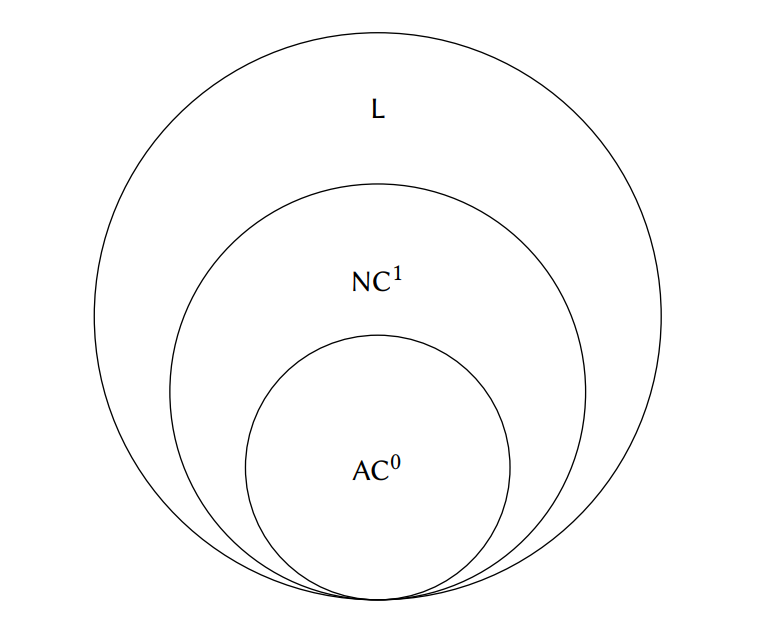
\includegraphics[scale=1]{ComplexityClasses.PNG}
\caption[]{The relationship between the complexity classes.\cite{lau2017computational}}
\label{complex}
\end{figure}
All these problems divide into complexity classes.
As the name suggests, the problems divide into classes that have approximately the same complexity.
The reduction of operations chooses the complexity class. For example, subtract can be reduced to add. 
We do this by changing the sign of the second input number with a negation gate. \\
In figure \ref{complex} the relationship between the complexity classes can be seen.
A nano-machine that solves the problems of the highest complexity class can also use the operations of the lower classes.
However, this does not work the other way around.
An L-machine can do logarithmic calculations as well as multiplications.
Though an $NC^1$-machine cannot do logarithmic calculations except it is $LOG_2$.  
In table \ref{table1} we can see the three different classes and the problems they may solve.
An L-machine can solve problems like a Turing machine. It also has a small amount of integrated memory.
The class $AC^0$ describes boolean circuits with polynomial-size and a constant depth, whereas the class $NC^1$ may have a logarithmic depth and two inputs per gate.\\ 
Problems can lower their class if researchers can find new reductions for them. 
However, problems exist that need more powerful machines or global knowledge about the network than an L-machine can offer.
Thus problems, like addressing, routing broadcasting/forwarding, could not be divided into the three complexity classes.
They are therefore not included in table \ref{table1}.\\
Insights into the feasibility of Nanao-machines provides the classification of the applications according to the computational power. 
Researchers may consult Table \ref{table1} to implement a protocol or an algorithm in a nano-machine. 
The algorithm must decompose into its basic operations. Afterward, the operation that is the most complex gives the decision for a complexity class.
Just because a nano-machine may perform only a few easy operations does not mean that it is simple to build, but the choice of complexity class can help.\\
Considering the $AC^0$ class, if a nano-machine can add, it may do all other operations of the complexity class.
Let us take the complexity class $NC^1$ for a practical example. In the human body, a nano-machine observes the concentration of a marker with $AVG$.
Since $THRES$ is also in the same class, this nano-machine can also check if a defined value exceeds. We can do this without increasing the complexity nor the memory.





\section{Conclusion}
This paper tries to close the gap of the insufficient specified computational requirements.
It does so by analyzing different scenarios. 
The analyzed problems divide into three complexity classes: $AC^0$, $NC^1$, $L$.
A nano-machine can then solve all the problems of his class and the class problems under him.\\
However, additional components, such as storage or clocking, may mean that the classes do not represent the actual implementation of the nano-machines.\\
Furthermore, we have not addressed the combination of operations, so the power of the complexity class may exceed.\\
In addition, the definition of extra complexity classes may specify the operations in more detail.







\bibliographystyle{acm}
\bibliography{sigproc} 

\end{document}
